\section{Wpływ funkcji nagrody}
\label{sec:wyniki-funkcja-nagrody}

Drugim elementem konfiguracji który analizowałem była funkcja nagrody. Porównałem bezpośredni
zysk netto z jego wersją przeskalowaną przy zachowaniu tego samego
algorytmu, reprezentacji stanu oraz seedu treningowego. Różnicę
zdefiniowałem jako

\begin{equation}
    \Delta EV_{\mathrm{reward}}
    =
    EV_{\mathrm{net}}
    -
    EV_{\mathrm{scaled}}.
\end{equation}

Ze wzoru wynika, że wartość dodatnia oznacza przewagę bezpośredniego zysku netto,
natomiast ujemna przewagę nagrody skalowanej. Wyniki wszystkich
czterech porównań przedstawiam w tabeli~\ref{tab:reward-effect}.

\begin{table}[htbp]
    \centering
    \caption{Wpływ funkcji nagrody na EV}
    \label{tab:reward-effect}
    \begin{tabular}{llrr}
        \toprule
        Algorytm & Reprezentacja & $\Delta EV_{\mathrm{reward}}$ & 95\% CI \\
        \midrule
        DQN & RAW
            & -0{,}0769 & [-0{,}1314,\ -0{,}0224] \\
        DQN & FEATURES
            & 0{,}0089 & [-0{,}0057,\ 0{,}0234] \\
        \midrule
        REINFORCE & RAW
            & 0{,}0018 & [-0{,}0087,\ 0{,}0124] \\
        REINFORCE & FEATURES
            & -0{,}0612 & [-0{,}1437,\ 0{,}0213] \\
        \bottomrule
    \end{tabular}
\end{table}

Dla DQN wykorzystującego reprezentację RAW cały przedział ufności leży
poniżej zera. Skalowanie nagrody poprawiło więc w tym wariancie 
wyniki końcowe w porównaniu z bezpośrednim wykorzystaniem
zysku netto. Sytuacja wyglądała inaczej po zastosowaniu reprezentacji
FEATURES, mianowicie różnica jest niewielka, a przedział obejmuje zero, dlatego na
podstawie tych wyników nie mogę wskazać wyraźnej przewagi jednej
z funkcji nagrody dla DQN korzystającego z tej reprezentacji.

Podobny brak zauważalnej przewagi wystąpił dla REINFORCE
z reprezentacją RAW, gdzie przedział ufności również obejmował zero.
Największą różnicę punktową dla REINFORCE zaobserwowałem przy
reprezentacji FEATURES, gdzie wyższy średni wynik osiągnęła funkcja
skalowana. Jednocześnie przedział ufności był tu bardzo szeroki, co
zgadzałoby się z dużym zróżnicowaniem końcowej jakości polityk REINFORCE
obserwowanym pomiędzy seedami.

Te same porównania przedstawiam także na rysunku~\ref{fig:reward-effect}. Na osi
poziomej znajduje się różnica $EV_{\mathrm{net}} -
EV_{\mathrm{scaled}}$, a na osi pionowej cztery kombinacje algorytmu
i reprezentacji stanu. Punkty przedstawiają średnią różnicę dla
pięciu sparowanych seedów treningowych, a wąsy 95-procentowe
przedziały ufności. W przeciwieństwie do wykresu wpływu reprezentacji
stanu, tutaj tylko jeden z czterech przedziałów, DQN z reprezentacją
RAW, leży całkowicie po jednej stronie zera.

\begin{figure}[htbp]
    \centering
    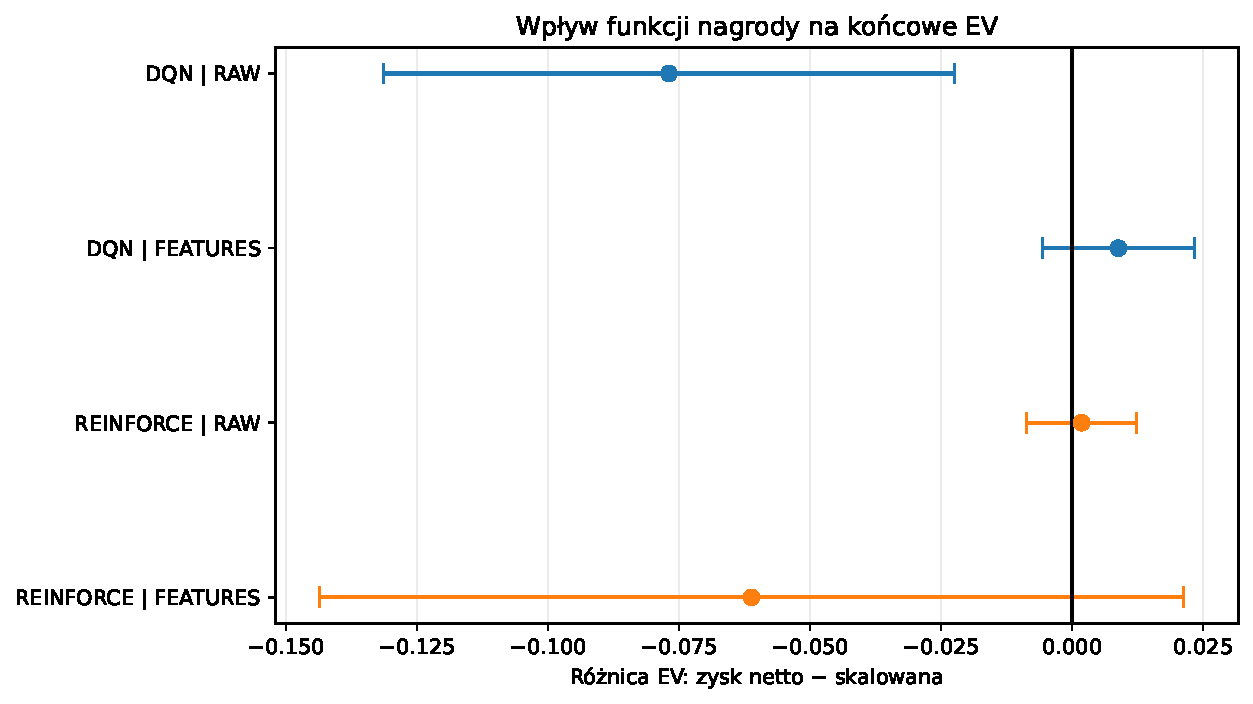
\includegraphics[
        width=0.9\textwidth
    ]{../experiments/results/final_analysis/03_reward_effect.pdf}
    \caption{Wpływ funkcji nagrody na końcowe EV.}
    \label{fig:reward-effect}
\end{figure}

W przeciwieństwie do reprezentacji stanu nie obserwuję więc efektu skalowania funkcji nagrody. 
Jej wpływ zależy od
połączenia z algorytmem oraz sposobem reprezentacji stanu. Skalowanie
poprawiło wyniki DQN korzystającego z reprezentacji RAW, lecz dla DQN
z reprezentacją FEATURES różnica była niewielka. W przypadku
REINFORCE punktowo najlepszy wynik uzyskała konfiguracja FEATURES ze
skalowaną nagrodą, ale wynik ten był jednocześnie silnie zależny od
seedu treningowego.
